\section{ХОД РАБОТЫ}

\subsection{Постановка задачи}

Создать оконное приложение, которое позволяло бы не только
выбирать записи из базы данных, но и добавлять и удалять их.

\subsection{Особенности разработанного приложения}

Для работы с sqlite Mono предоставляет следующие классы из пространства имен
\texttt{Mono.Data.Sqlite}:

\begin{itemize}
\item \texttt{SqliteConnection};
\item \texttt{SqliteCommand};
\item \texttt{SqliteDataReader};
\item \texttt{SqliteException}.
\end{itemize}

Класс \texttt{SqliteConnection} используется для установки соединения с базой данных,
\texttt{SqliteCommand} представляет собой объект SQL-запроса, 
\texttt{SqliteDataReader} используется для чтения строк данных, 
полученных при выполнении запроса SELECT, а класс \texttt{SqliteException}
используется для представления различных ошибок взаимодействия с sqlite в виде объектов C\#. 

На рисунке~\ref{lst:sqlite_select} представлен пример запроса на выборку данных,
реализованный с помощью вышеупомянутых классов.

\begin{lstlisting}[caption=Пример запроса на выборку данных,
label=lst:sqlite_select,language={Java},basicstyle=\scriptsize\ttfamily]
try {        
    dbConnection.Open();

    String queryString = String.Format("SELECT Description FROM Books WHERE Title='{0}'",
                                       bookTitle);
        
    using (SqliteCommand cmd = new SqliteCommand(queryString, dbConnection)) {
        using (SqliteDataReader rdr = cmd.ExecuteReader()) {
            rdr.Read();
            bookDescription = rdr["Description"].ToString();
          }
      }
  }
catch (SqliteException ex) { Console.WriteLine(ex); }
finally { dbConnection.Close(); }
\end{lstlisting}

Интересной особенностью sqlite является тот факт, 
что для указания того, что данные имеют строковый тип,
используются одинарные кавычки,
поэтому при изменении строковых данных необходимо
предварительно экранировать все одинарные кавычки.

На рисунке~\ref{pic:interface} приведен пользовательский интерфейс
разработанного приложения.

\begin{figure}[h!]
  \centering
  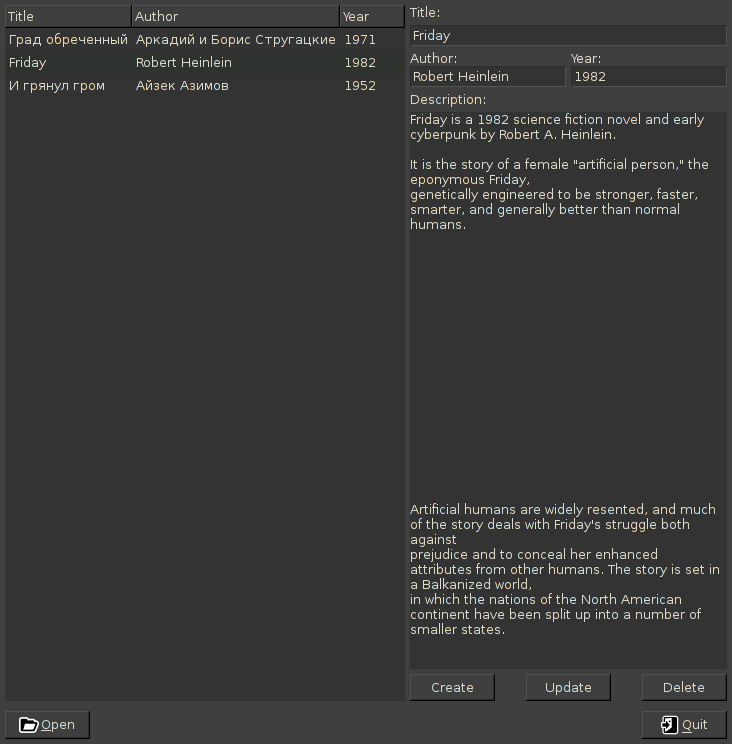
\includegraphics[width=150mm]{pic/interface}
  \caption{Интерфейс разработанного приложения}
  \label{pic:interface}
\end{figure}

Исходный текст разработанного приложения находится в приложении~А.